
\title{Building a Probablistic Graphical Model for Human-Wildife Conflict}

\author{Chavoux Luyt}
\maketitle
\begin{abstract}
Although many methods has been suggested to mitigate human-predator
conflict, it is still a worldwide and increasingly important problem,
both for predator conservation and for livestock farming. In the past
most solutions to this conflict has been either from an agricultural
perspective or from a conservation perspective. However, because the
goals of these two perspectives are seldom the same, there has been
frustratingly little progress in preventing human-wildlife conflict.
Here we review different published methods used worldwide to alleviate
human-wildlife conflict, specifically conflict between livestock farmers
and predators, the pros and cons of each method and the probable usefulness
of the different methods to livestock farmers in North Central Namibia.
We propose a more useful classification of methods than the usual
lethal non-lethal dichotomy, and compare the various methods in terms
of their success and cost-effectiveness. We also investigate the possible
reasons for both failures and successes of the different methods.
Lastly we propose that a new approach is needed if we want practical
and sustainable solutions to our current human-wildlife conflicts.
\end{abstract}

\section{Introduction}

\paragraph{Human-wildlife conflict is a growing global problem \citep{Messmer_2000,Treves_n_Karanth_2003b,Nyhus_et_al_2005}.
Land managers, specifically farmers, are key to finding sustainable
solutions to this conflict. One major reason why attempts at mitigating
farmer-predator conflict in the past have failed, is because the local
conditions on a specific farm has not been taken into account sufficiently.
And farmers did not always have the relevant information available
to decide on the best management strategy that will be both cost-effective
and sustainable in the long run. }

\paragraph{Farmlands are part of a wider ecosystem. Therefore both the ecological
sustainability and the agricultural cost-effectiveness of any proposed
solution, are critical to its success. Typically, ecological modelling
has fallen into two broad groups. Simulation models typically tries
to incorporate as many different parameters as possible and to be
as realistic as possible. Because of the huge number of parameters,
some of which might not be relevant, these kind of models often end
up as a \textquotedbl{}black box\textquotedbl{} with little guarantee
that it is actually true to the real situation and that all the relevant
factors have been included in the model. It is often no longer understandable
from a human perspective. The opposite approach is to simplify matters.
It is accepted that the model is not realistic representation of ecosystem.
Instead, the aim of the model is to gain a better understanding of
the ecosystem. It is a conditional model, basically saying that \textit{if
}certain conditions and assumptions are true \textit{then }certain
effects can be expected to result from it. It ignores all other influences
by concentrating only on those parts of the model that is relevant
to the specific question being asked. In the process, the model is
kept simple enough that it can be understood by humans.}

\paragraph{For livestock farmers to decide on the best solution for preventing
livestock depredation in their specific situation, it is important
that they are able to trust the output of a specific model. For this
reason, a model that is humanly understandable is more useful than
a possibly more realistic, but incomprehensible model. It is also
important that those agricultural aspects of the farming enterprise
that will play an important role in their decision, are included in
the model. Farmers are having to survive in uncertain circumstances
and explicit recognition of the uncertainty that is part of all farming,
can also help them to realize the limitations of management decisions
based on uncertain facts.}

\section{Why use Probabilistic Graphical Models (PGMs)?}

\paragraph{Our knowledge of farmland ecosystems are incomplete and thus necessarily
bound up with uncertainty. Historically there has been three approaches
to modelling uncertainty in computer systems:}
\begin{enumerate}
\item Fuzzy logic. Here statements are not considered as either true (1)
or false (0), but as having a certain degree of truth between 0 and
1, resulting in a multi-valued logic. This result in the counter-intuitive
result that f(A \ensuremath{\bigvee} \textlnot{} A) \ensuremath{\neq}
f(True). Whereas normally either a statement A or its negation NOT
A, would be true, this is not necessarily true in fuzzy logic. As
a result, although fuzzy logic based expert systems have been very
successful in commercial applications, these have tended to be rather
small, with limited levels of inference, and the various parameters
often need to be tuned using machine learning techniques. The fact
that it includes some obviously counter-intuitive statements, makes
it difficult to understand or explain and thus not really a good choice
for our use case. Additionally, farming systems and ecosystems are
complicated, making it difficult to model using fuzzy logic that are
better suited to smaller systems.
\item Dempster-Shafer modelling is another approach to dealing with uncertainty.
Instead of dealing directly with probabilities though, it deals with
the degree of evidence we have for certain truth values, called belief
functions. This can be a very useful approach in some circumstances.
However, the theoretical basis of this model and the situations for
which it is a good fit, are still debated. It is best used when there
are multiple independent sources of evidence with some overlap concerning
the same basic question (i.e. an accumulation of evidence). Because
it looks only at evidence, rather than at probabilities, it cannot
deal directly with cause and effect. It has been considered as a generalization
of probabilistic theory, and can be simpler to implement than the
Bayesian Network approach. However, it has no way to model cause and
effect naturally, and can only combine various pieces of evidence
for a certain outcome, without implying any causal relationship. One
possible advantage of this approach, is that an explicit value can
be assigned to uncertainty. However, it is easily misused for situations
where it is not a good fit and can give counter-intuitive or untrustworthy
results in such cases \citep{Josang_et_al_2010}.
\item Bayesian probability theory has a long history and is much better
understood than the previous two approaches from a mathematical point
of view. One important advantage compared to the other two types of
models, is that it provides a very natural method to model dependencies
and conditional dependencies, making it very intuitive to model real
cause and effect relationships between different factors. However,
it can be computationally expensive. Until recently, it was impossible
to model the joint probability distribution over any reasonable number
n of random variables taking x different values per variable. It would
require $x^{n}$ different probability assignments, which are both
computationally expensive and too large to fit into computer memory,
and incomprehensible to the human brain \citep{Koller_n_Friedman_2005}.
This remained the main barrier to using probabilistic methods for
solving problems dealing with uncertainty, until fairly recently when
the current methods of Probabilistic Graphical Models (PGMs) were
developed. The recent developments have resulted in PGMs based on
Bayesian probability theory becoming the dominant paradigm in most
modern expert systems in general and decision support systems in particular
\citep{Koller_n_Friedman_2005}. For these reasons, this approach
was chosen as the preferred one for modelling the different human-wildlife
mitigation methods.
\end{enumerate}

\paragraph{There are many different Probabilistic Graphical Models, but the
best fit for the kind of problem we are looking to solve for farmer-predator
conflict, would be a version of Bayesian Network (Koller 2016, personal
communication). A Bayesian Network is a Directed Acyclical Graph (DAG),
consisting of a number of nodes, representing random variables, connected
by directed edges, representing dependencies between the nodes and
a table with the conditional probability distribution for each node
given its parents. For the marginally independent nodes (those without
any parents) their probabilities are given by a prior probability
distribution. The basic Bayesian Network has been extended to a form
known as Influence Diagrams. In this type of model, not only the various
random variables and their conditional probability functions are described,
but additionally, there are }
\begin{enumerate}
\item action variable nodes, denoting actions that can be taken by humans
and 
\item utility nodes, denoting the expected utility that will result from
the chosen action.
\end{enumerate}

\paragraph{Running the model for each choice of anti-depredation method, a Maximum
Expected Utility (MEU) value can be calculated for that method. While
this MEU might not be an exact value denoting the true maximum expected
utility of each choice, it is robust for comparing the different methods,
since essentially the same model is used for each method and just
the parameters change, depending on the method. As in any other computer
program, the GIGO (garbage in, garbage out) principle still holds,
however. The results would still be dependent on the reliability of
the data provided by the farmer and the robustness of the assumptions
built into the model. Using a Probabilistic Graphical Model however,
the assumptions are stated explicitly as part of the model and can
be updated over time in order to improve the model.}

\section{The model - What data do we need to make an informed and useful decision?}

\paragraph{For livestock farmers to make an informed decision on the best anti-predation
method for their specific circumstances, both ecological and agricultural
information should be used. From a strictly (and short-term) agricultural
point of view, the cost and relative efficiency of the different methods
used to protect livestock from predation should be the most important
factor. Other agricultural aspects to be considered, include the available
infra-structure on the land, the availability of capital for farm
infrastructure improvements, the sustainable stocking rates of the
land, the long-term effects of the different techniques on the veld
quality, the kind and breeds of livestock (and the marketing and other
reasons for using these specific types), the topography and vegetation
types of the land, the density of available water points and the quality
and quantity of drinking water on the land, the size of the farm,
etc. }

\paragraph{However, especially for the long-term sustainability of whichever
method is used, a number of ecological aspects are important as well.
Two question concerning predator diet preferences can influence the
management of a livestock farmer: }
\begin{enumerate}
\item The diet preferences (if any) of the predator species on his farm
impacting livestock or game production (i.e. if he can stock the farm
with cheaper, but preferred prey species, his high-value game or livestock
animals are less likely to be preyed on by these predators) and 
\item the importance of individual prey preference of the predators on his
land (i.e. if there are only some individuals that are preferring
livestock as prey, removing them from his land might be a viable management
option). 
\end{enumerate}

\paragraph{The habitat preferences of predators can influence his management
options in two ways: }
\begin{enumerate}
\item If different predator species (that prey on different kinds of livestock
or age classes) prefer different habitat types, it may be possible
to keep vulnerable livestock away from those high-risk habitats on
his farm (provided there is enough low-risk alternative areas available)
and 
\item if the reason why certain predators prefer certain habitat types within
their wide-ranging home ranges can be established (e.g. for hunting,
or by females with higher prey requirements for having their cubs),
vulnerable livestock can be kept away from these habitats. 
\end{enumerate}

\paragraph{Lastly, the interactions between the predator species can also influence
management options. It has been claimed that caracals can deter jackals
from some areas \citep{DuToit_2013} and it is known that leopards
will kill and eat blackjacked jackals \citep{Bothma_n_Le_Riche_1994},
and that caracals and jackals will occasionally kill each other's
young. One of the major reasons for the increasing problems with jackals
and caracals could be meso-predator release \citep{Beinart_1998},
but the extend and importance of these interactions have not been
studied in enough detail to know if it could be a significant reason
for the reported increase in livestock depredation. If meso-predator
release plays a role in Namibian ecosystems, it becomes important
for farmers to maintain enough larger predators on their land to prevent
future livestock losses from too many meso-predators.}
\begin{description}
\item [{A}] conceptual Bayesian Network model:
\begin{figure}[h]
\textit{\caption{Conceptual PGM to determine success probability of farmer-predator
conflict resolution methods. Grey nodes indicate data we need from
the farmer, white nodes the pre-existing model. The final value is
a probability that a specific method will be successful for a specific
farmer.}
}
\begin{description}
\item [{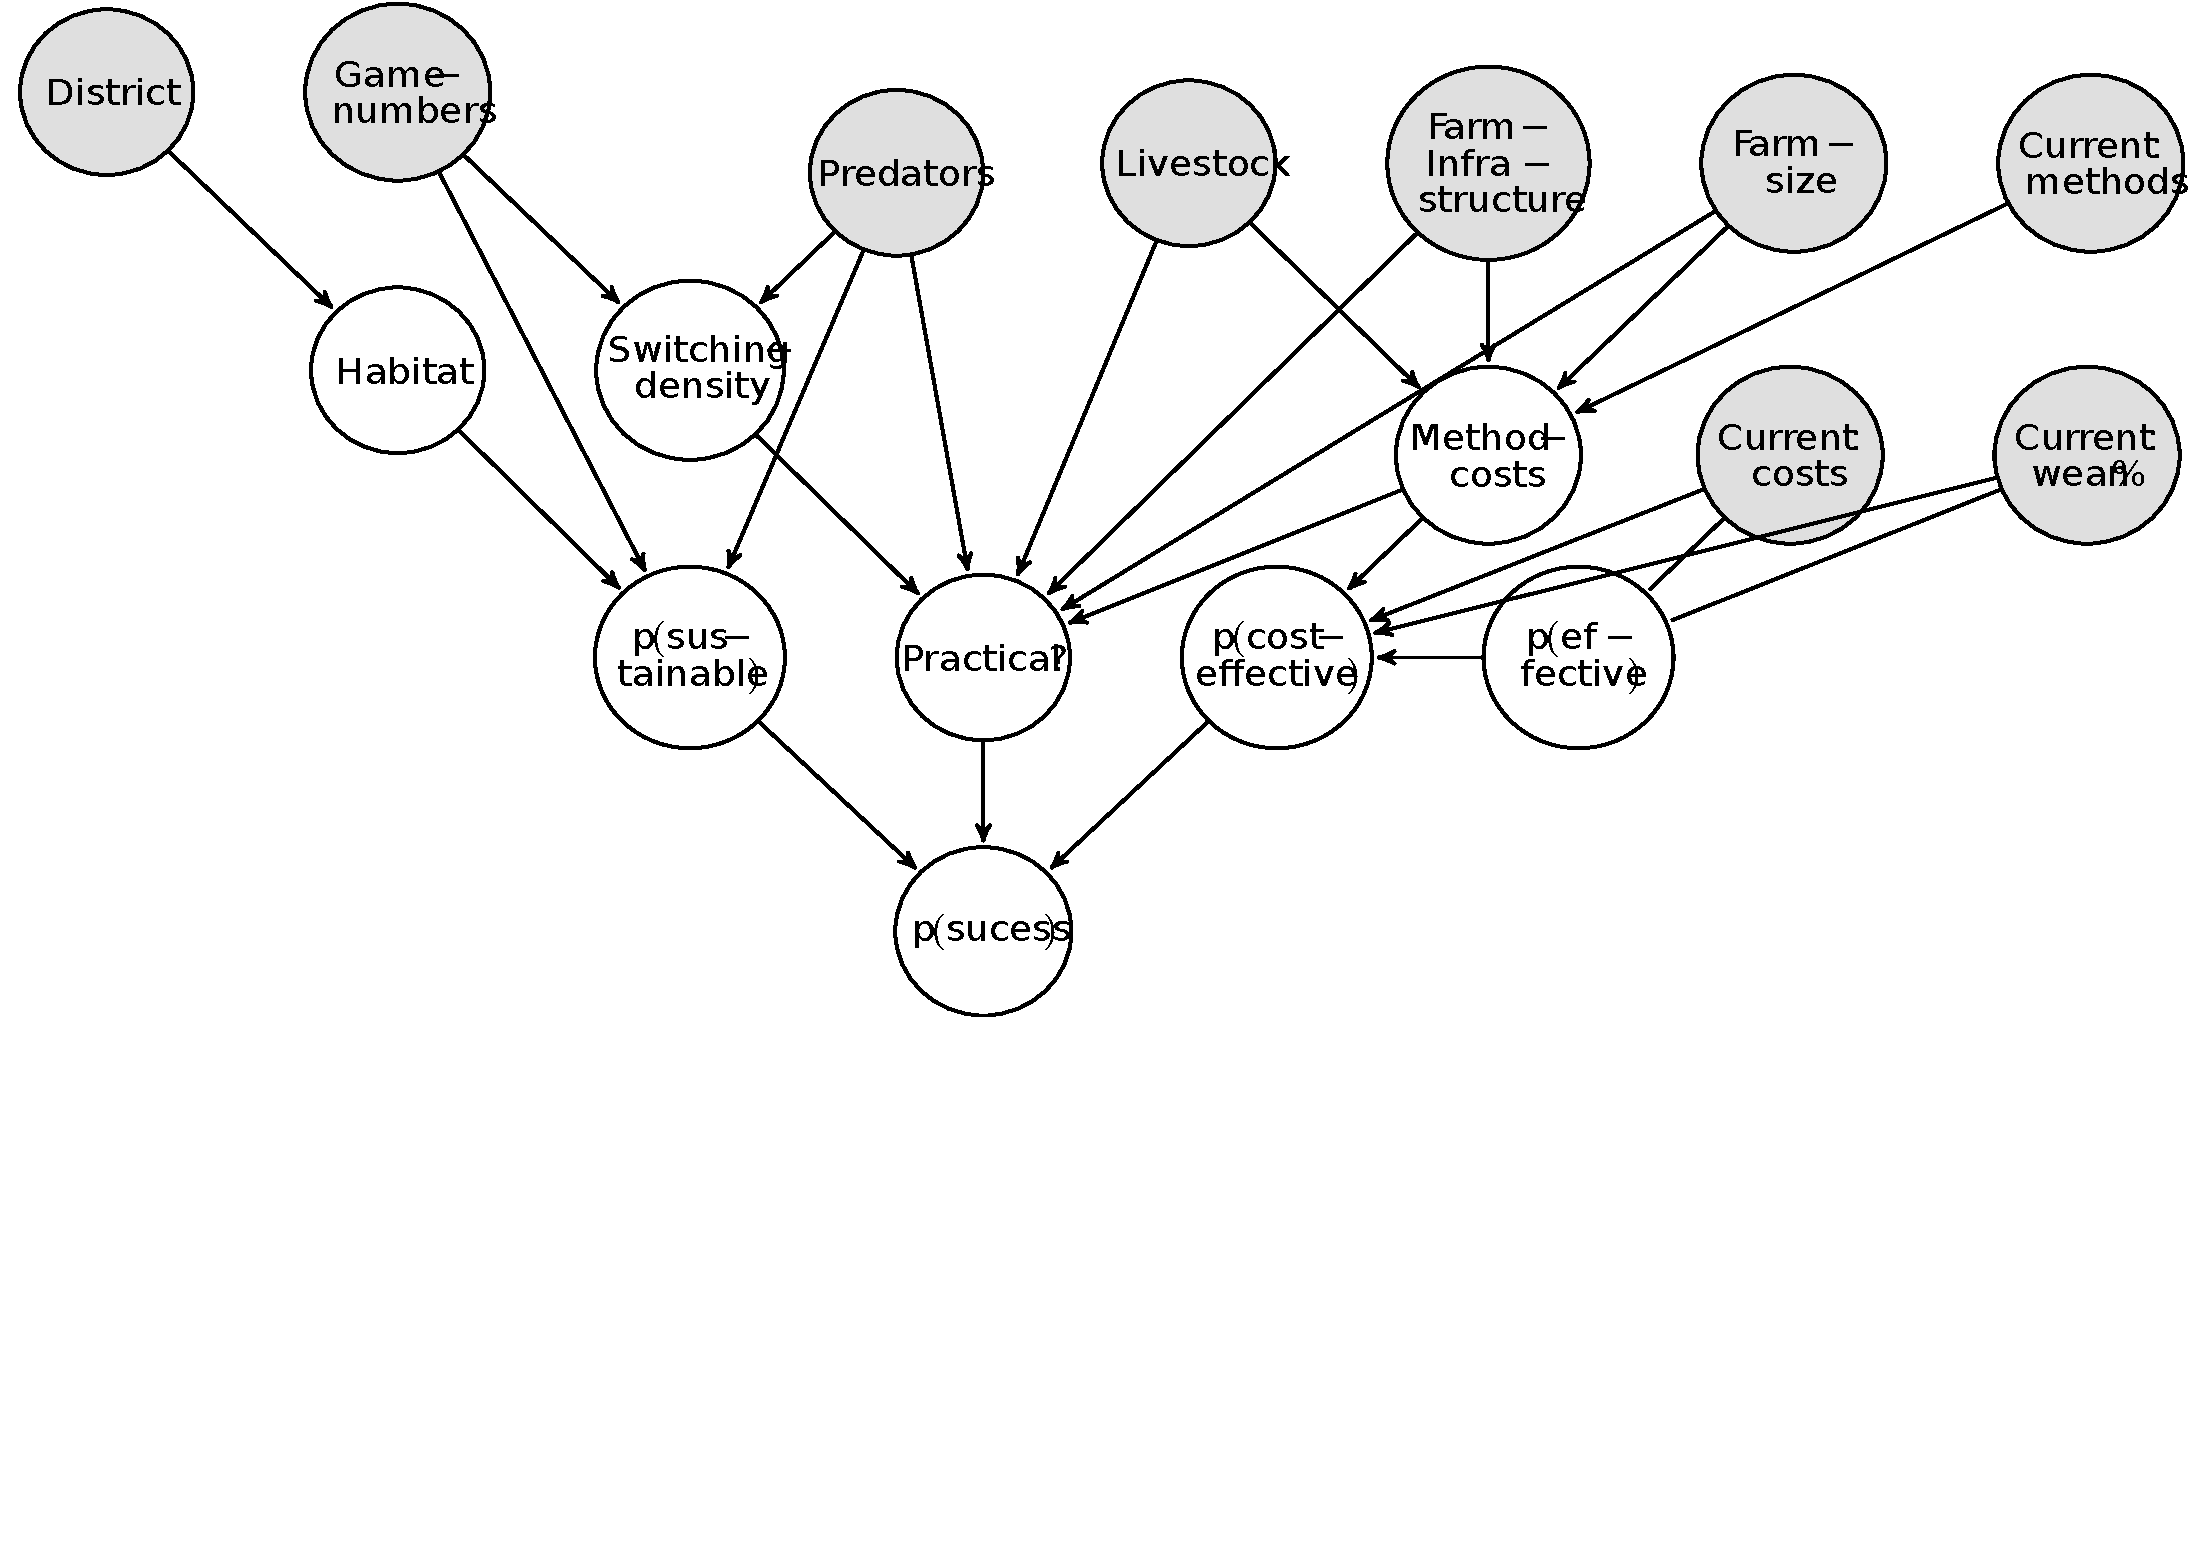
\includegraphics[width=0.8\paperwidth]{/home/boer/doks/PhD/Tesis/Images/FwP_Model}}]~
\end{description}
\end{figure}
\end{description}

\section{Constraints and limitations}
\begin{description}
\item [{What}] kind of data (which would be really useful) is unavailable
currently and in the foreseeable future? What are the uncertainties?
How can we work around these uncertainties to still get useful answers?
GIGO (Garbage in, garbage out): How do we prevent \textquotedbl{}garbage
data\textquotedbl{} from fouling our model? How can we adapt our model
to changing circumstances? How can we extrapolate the model to other
species and situations (e.g. more predator species, communal farmers,
other continents and biomes)?
\end{description}

\section{Refining our model}
\begin{description}
\item [{Using}] data from farmers using the online Decision Support System
to update our model automatically. Providing an easy way to update
our parameters as more research becomes available. Writing a transparent
model and keeping it simple enough to understand and update (the KISS
principle). Using alternative algorithms (e.g. Dempster-Shafer to
deal with uncertainty instead of pure Bayesian Networks). Open Source.
\end{description}

\section{Conclusions}

\paragraph{Many different approaches to human-wildlife conflict have been used
in the past, with partial success. Many farmers still prefer to kill
predators on their land or to engage in unsustainable farming practices,
without the issue being resolved. Human-wildlife conflict still remain
the major cause of death for many predators, but ultimately farmers
remain the custodians of predators on their land and need to be empowered
to do a better job of managing their land, including both agricultural
aspects and ecological aspects of farmer-predator conflict. An online
decision support system can put the relevant knowledge into the hands
of farmers who are struggling with livestock depredation on their
land. It can also be updated periodically, making sure that it remains
current. In time, the model can be expanded or adapted to include
communal farming systems \citep{Blackburn_et_al_2016} and other predators.}

\bibliographystyle{/home/boer/TeX/bibtex/bst/stellenbosch/myplainnat}
\bibliography{/home/boer/doks/PhD/Literature/Ecology}

